\begin{titlepage}
  \begin{center}
    {\Huge\textsc{Johns Hopkins University}\par}
    \vspace*{\stretch{1}}
    {\Huge\textbf{\DocumentAuthor}\par}
    \vspace*{\stretch{1}}
    \begin{center}
      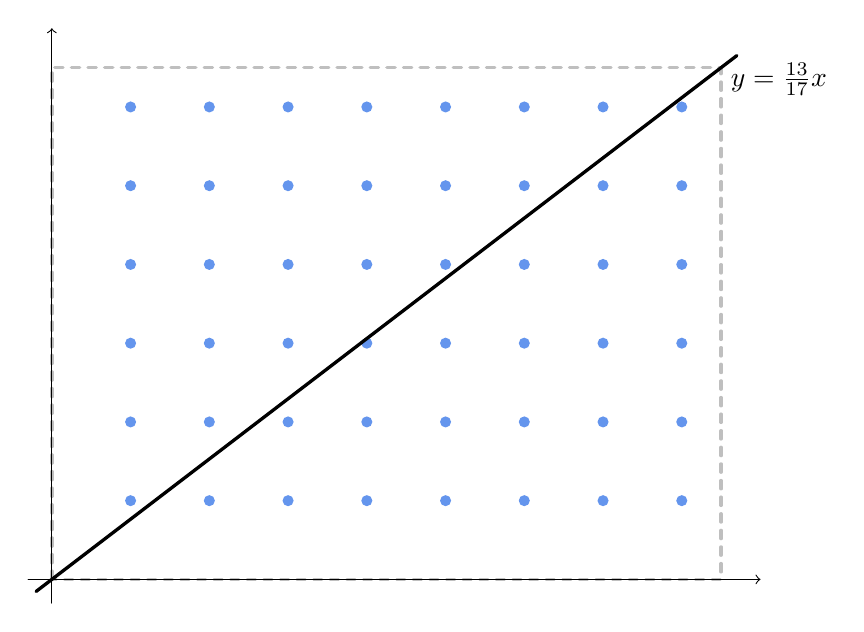
\begin{tikzpicture}[scale=1,line join=round,line cap=round]
        
        \def\p{17}
        \def\q{13}
        \def\xmax{8.5}
        \def\ymax{6.5}
        
        \draw[very thick,lightgray,dashed] (0,0) rectangle (\xmax,\ymax);
        
        \draw[->] (-0.3,0) -- (\xmax+0.5,0);
        \draw[->] (0,-0.3) -- (0,\ymax+0.5);
        
        \foreach \x in {1,2,3,4,5,6,7,8} {
          \foreach \y in {1,2,...,6} {
            \fill[CornflowerBlue] (\x,\y) circle (2pt);
          }
        }
        
        \draw[very thick, domain=-0.2:\xmax+0.2] plot (\x, {(\q/\p)*\x});
        
        \node[right,yshift=-1ex] at (\xmax,\ymax) {$y=\frac{13}{17}x$};    
      \end{tikzpicture}

    \end{center}
    \vspace*{\stretch{.5}}
    {\superhuge \textbf{\VolumeTitle}\par}
    \vspace*{\stretch{1}}
    {\Large Book II of\par}
    \vspace*{\stretch{.5}}
    {\huge \textsc{\SeriesTitle}\par}
    \vspace*{\stretch{2}}
    {\Large\Version{0}}
  \end{center}
\end{titlepage}
